%\title{LaTeX Portrait Poster Template}
%%%%%%%%%%%%%%%%%%%%%%%%%%%%%%%%%%%%%%%%%
% a0poster Portrait Poster
% LaTeX Template
% Version 1.0 (22/06/13)
%
% The a0poster class was created by:
% Gerlinde Kettl and Matthias Weiser (tex@kettl.de)
% 
% This template has been downloaded from:
% http://www.LaTeXTemplates.com
%
% License:
% CC BY-NC-SA 3.0 (http://creativecommons.org/licenses/by-nc-sa/3.0/)
%
%%%%%%%%%%%%%%%%%%%%%%%%%%%%%%%%%%%%%%%%%

%----------------------------------------------------------------------------------------
%	PACKAGES AND OTHER DOCUMENT CONFIGURATIONS
%----------------------------------------------------------------------------------------

\documentclass[a0,portrait]{a0poster}

\usepackage{multicol} % This is so we can have multiple columns of text side-by-side
\columnsep=100pt % This is the amount of white space between the columns in the poster
\columnseprule=3pt % This is the thickness of the black line between the columns in the poster

\usepackage[svgnames]{xcolor} % Specify colors by their 'svgnames', for a full list of all colors available see here: http://www.latextemplates.com/svgnames-colors

\usepackage{times} % Use the times font
%\usepackage{palatino} % Uncomment to use the Palatino font

% Justify
\usepackage{ragged2e}

% Titles
\usepackage{titlesec}
\titleformat*{\section}{\LARGE\bfseries\filcenter}
\titleformat*{\subsection}{\Large\bfseries\filcenter}
\titleformat*{\subsubsection}{\large\bfseries\filcenter}
\titleformat*{\paragraph}{\large\bfseries\filcenter}
\titleformat*{\subparagraph}{\large\bfseries\filcenter}
\titlespacing\section{0pt}{14pt}{6pt}
\titlespacing\subsection{0pt}{0pt}{0pt}

\usepackage{enumitem}
\newenvironment{nitemize}{%
  \begin{itemize}[topsep=6pt,itemsep=2pt,parsep=0pt]%
}{%
  \end{itemize}%
}
\newenvironment{nenumerate}{%
  \begin{enumerate}[topsep=6pt,itemsep=2pt,parsep=0pt,label=\textbf{\arabic*. }]%
}{%
  \end{enumerate}%
}

\usepackage{graphicx} % Required for including images
\graphicspath{{figures/}} % Location of the graphics files
\usepackage{booktabs} % Top and bottom rules for table
\usepackage[font=small,labelfont=bf]{caption} % Required for specifying captions to tables and figures
\usepackage{amsfonts, amsmath, amsthm, amssymb} % For math fonts, symbols and environments
\usepackage{wrapfig} % Allows wrapping text around tables and figures
\newenvironment{Figure}
  {\par\medskip\noindent\minipage{\linewidth}}
  {\endminipage\par\medskip}

\let\OLDthebibliography\thebibliography
\renewcommand\thebibliography[1]{
  \OLDthebibliography{#1}
  \setlength{\parskip}{0pt}
  \setlength{\itemsep}{0pt plus 0.1ex}
}

\begin{document}

%----------------------------------------------------------------------------------------
%	POSTER HEADER 
%----------------------------------------------------------------------------------------

\begin{figure}[!htb]
\minipage{0.33\textwidth}
  \begin{flushleft}
  \includegraphics[height=0.03\textheight,keepaspectratio]{ICL.eps}
  \end{flushleft}
\endminipage\hfill
\minipage{0.33\textwidth}
  \centering
  \includegraphics[height=0.03\textheight,keepaspectratio]{CDT.png}
\endminipage\hfill
\minipage{0.33\textwidth}%
  \begin{flushright}
  \includegraphics[height=0.03\textheight,keepaspectratio]{EPSRC.png}
  \end{flushright}
\endminipage
\end{figure}
\vspace{0.2cm}
\centering
\veryHuge \color{Black} \textbf{Computational model for the modulation of speech-in-noise comprehension through transcranial electrical stimulation} \color{Black}\\[0.5cm] % Title
\huge \textbf{Mikolaj A. Kegler\textsuperscript{1,2}, Tobias Reichenbach\textsuperscript{1,2}}\\[0.4cm] % Author(s)
\Large \textsuperscript{1}Department of Bioengineering, \textsuperscript{2}Centre for Neurotechnology\\Imperial College, South Kensington, SW7 2AZ, London % University/organization
% \end{minipage}
%
% \begin{minipage}[b]{0.25\linewidth}
% \includegraphics[width=20cm]{logo.png}\\
% \end{minipage}

\vspace{0.4cm} % A bit of extra whitespace between the header and poster content

%----------------------------------------------------------------------------------------

\begin{multicols*}{2} % This is how many columns your poster will be broken into, a portrait poster is generally split into 2 columns

%----------------------------------------------------------------------------------------
%	INTRODUCTION
%----------------------------------------------------------------------------------------
\section*{\underline{Introduction}}
\begin{flushleft}
\normalsize
Transcranial electrical stimulation (TES) can non-invasively modulate neuronal activity in humans. Recent studies have shown that TES with an alternating current that follows the envelope of a speech signal can modulate the comprehension of this voice in background noise \cite{Wilsch2018TranscranialComprehension}. However, how exactly it influences the cortical activity and improves speech comprehension remains poorly understood.
\end{flushleft}

%----------------------------------------------------------------------------------------
%	OBJECTIVES
%----------------------------------------------------------------------------------------

\section*{\underline{Objectives}}
\begin{flushleft}
\normalsize
\begin{nenumerate}
\item Establish a biologically plausible computational model of spiking neural network reflecting natural speech encoding in the auditory cortex.
\item Assess the network's speech-in-noise encoding performance considering different levels of background multi-talker babble noise.
\item Investigate the effect of different external currents on the network dynamics and optimize the stimulation paradigm for the enhancement of natural speech processing.
\end{nenumerate}
\end{flushleft}

%----------------------------------------------------------------------------------------
%	MATERIALS AND METHODS
%----------------------------------------------------------------------------------------

\section*{\underline{Materials and Methods}}
\subsection*{Computational model \textnormal{(adapted from \cite{Hyafil2015a})}}
\begin{Figure}
\centering
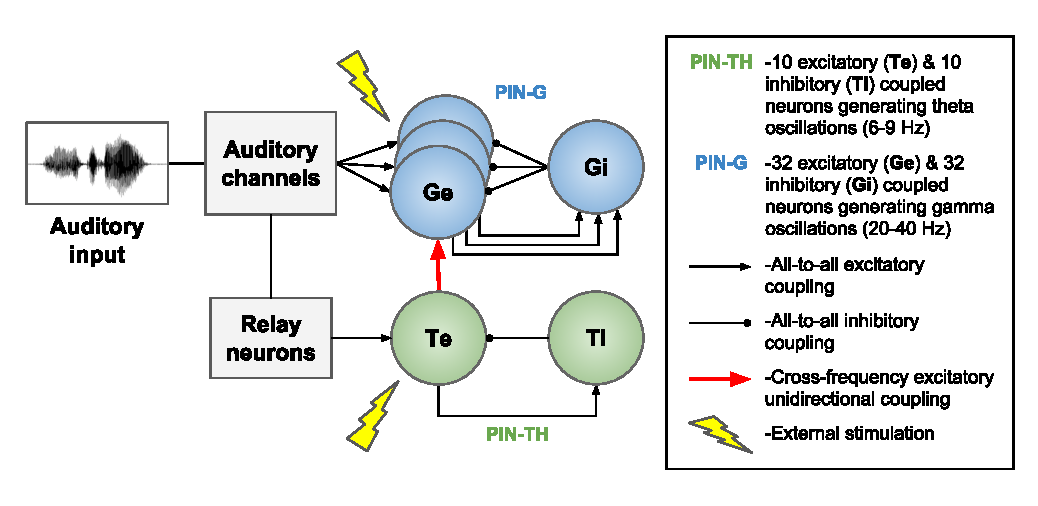
\includegraphics[width=\linewidth,keepaspectratio]{Architecture.eps}
\end{Figure}
\begin{flushleft}
\normalsize
\begin{nitemize}
\item \textbf{Auditory channels}: the subcortical auditory processing model \cite{Chi2005MultiresolutionSounds} decomposes auditory input into 32 distinct frequency bands (90-3623 Hz).
\item \textbf{Relay neurons}: a population of neurons that project the auditory channels with a delay of up to 50 ms and weights that represent the strength of synaptic connections.
\item \textbf{External stimulation}: tDCS, sine-wave tACS and speech envelope shaped current at different phase lags and intensity levels were delivered to $Ge$ and $Te$ populations.
\end{nitemize}
\begin{Figure}
\centering
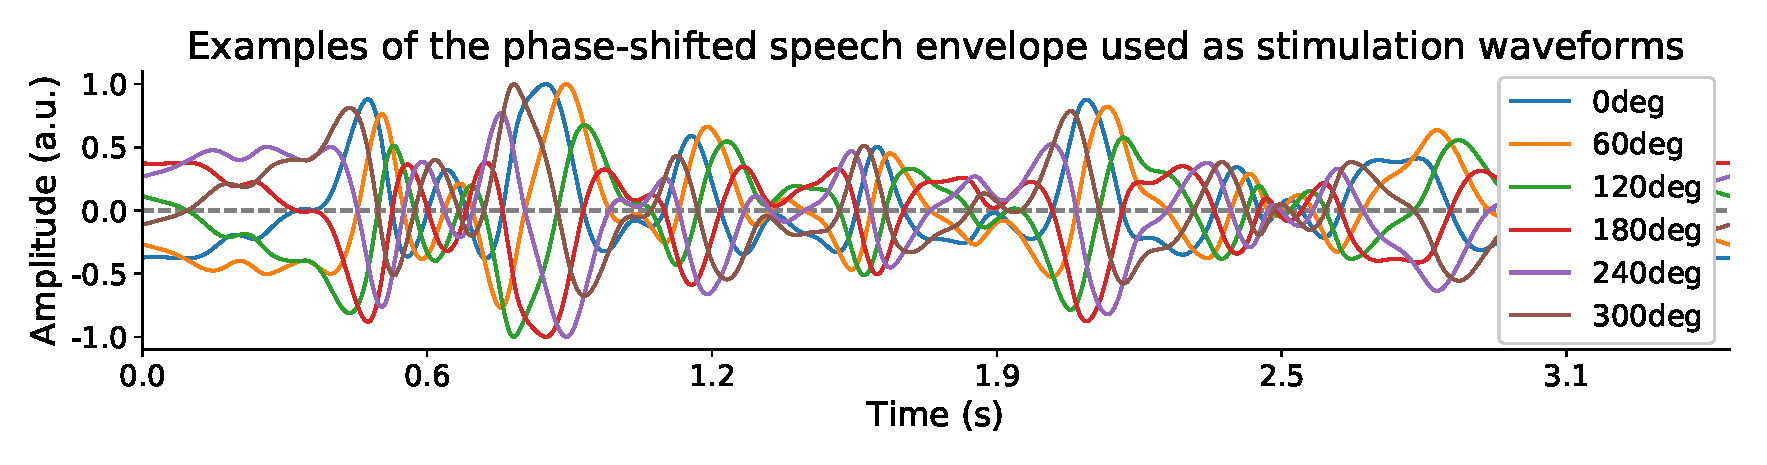
\includegraphics[width=\linewidth,keepaspectratio]{Envelopes.eps}
\end{Figure}
\end{flushleft}

\subsection*{Syllable decoding}
\begin{flushleft}
\begin{Figure}
\centering
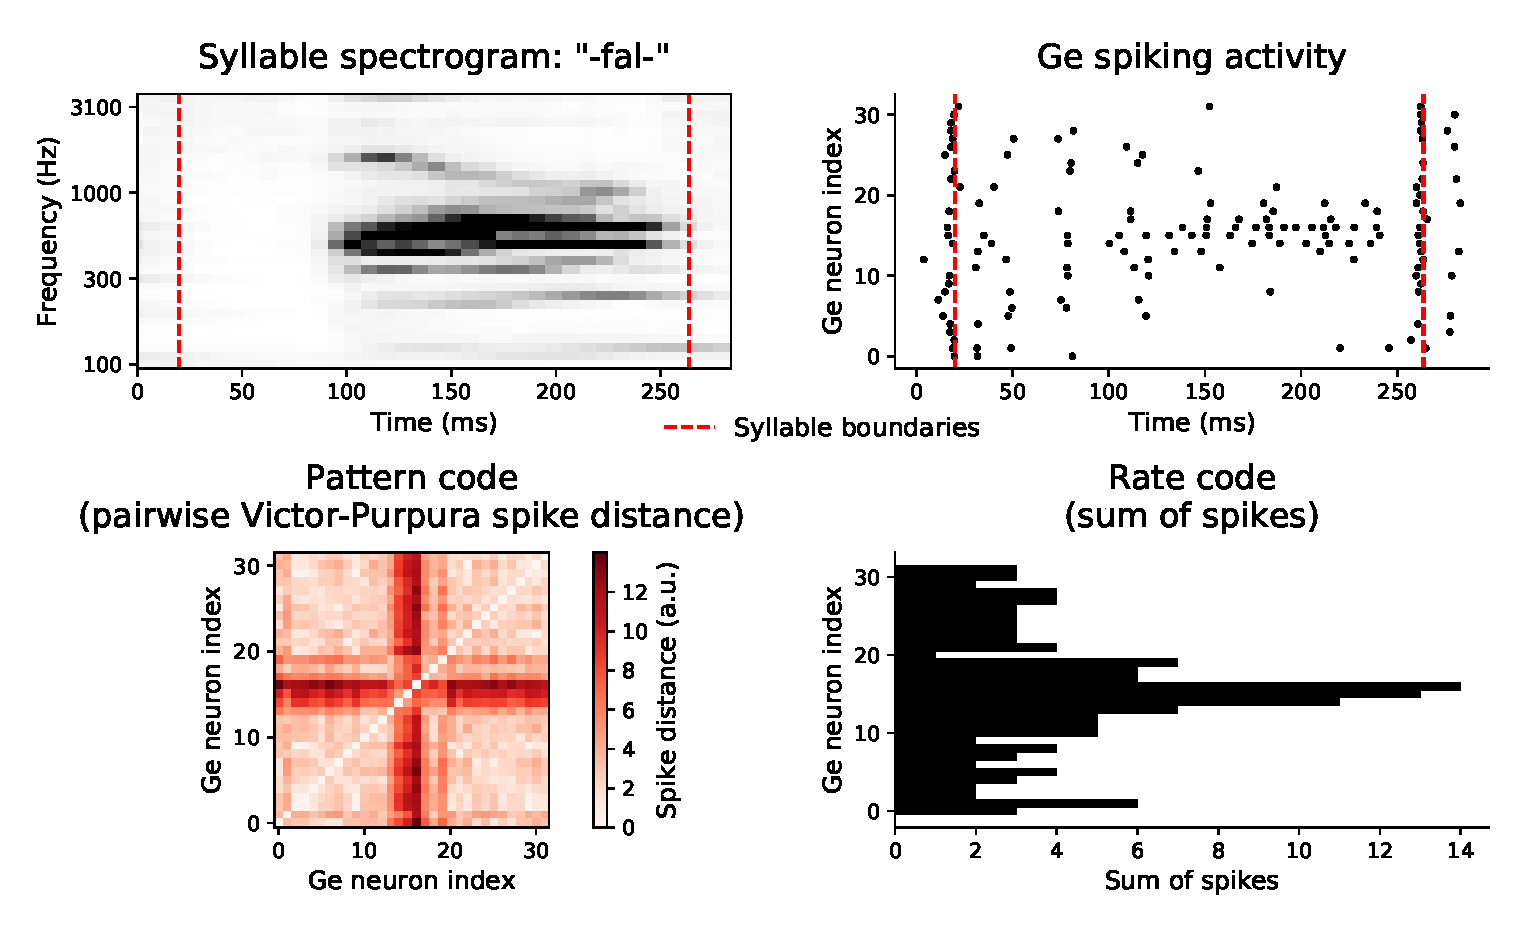
\includegraphics[width=\linewidth,keepaspectratio]{Encoding.eps}
\end{Figure}
\normalsize
\begin{nitemize}
\item 100 sentences from \textbf{TIMIT} database, each preceded by 500-1500 ms of silence, were presented to the model 100 times each. A single \textbf{classification trial} was performed using a random subset of \textbf{10 syllables} from all the available.
\item \textbf{Onsets of syllables} were indicated by spike bursts in the PIN-TH network.
\item \textbf{Nearest centroid algorithm} was used to decode syllables based on \textbf{pattern} or \textbf{rate code} obtained from the model simulations. To decode syllables from speech-in-noise, the centroids were obtained from the simulations employing the same sentences but \textbf{without masking noise}.
\item \textbf{200 classification trials} were obtained for each of the considered levels of masking \textbf{babble noise}. 
\item To seek for the similarity with normal human performance in speech-in-noise listening task a \textbf{sigmoid function} was fitted to all the obtained results to determine at what level of SNR the algorithm yields \textbf{50\% relative decoding accuracy}.
\end{nitemize}
\end{flushleft}

%----------------------------------------------------------------------------------------
%	RESULTS
%----------------------------------------------------------------------------------------

\section*{\underline{Results}}
\subsection*{Network's behavior \textnormal{(without external stimulation)}}
% \minipage{0.7\linewidth}
% \centering
% 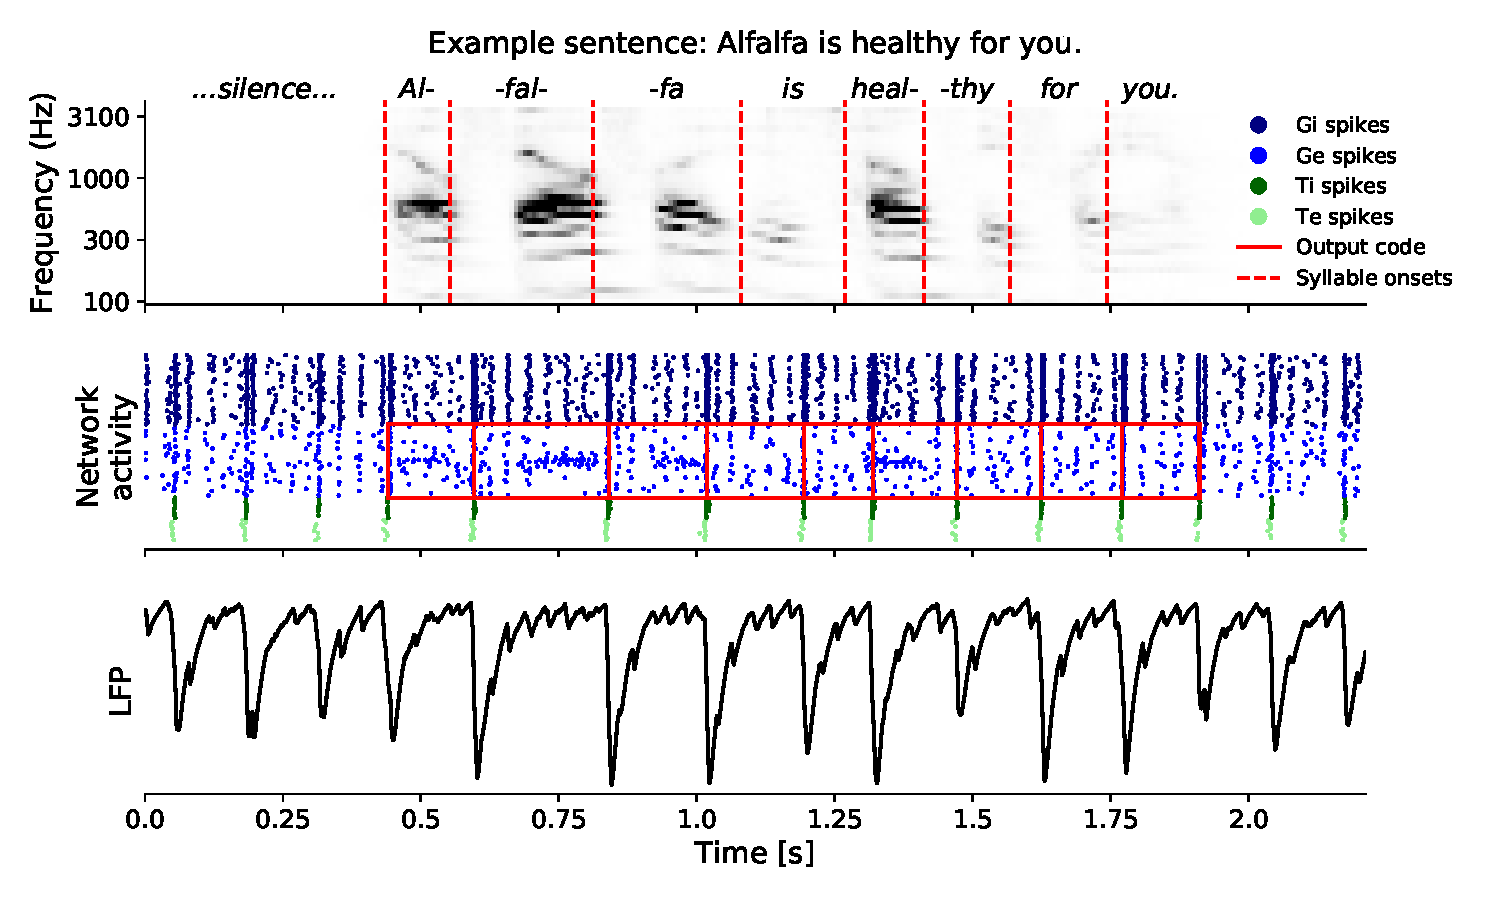
\includegraphics[width=\linewidth,keepaspectratio]{Behaviour.eps}
% \endminipage\hfill
% \minipage{0.3\linewidth}%
% \centering
% 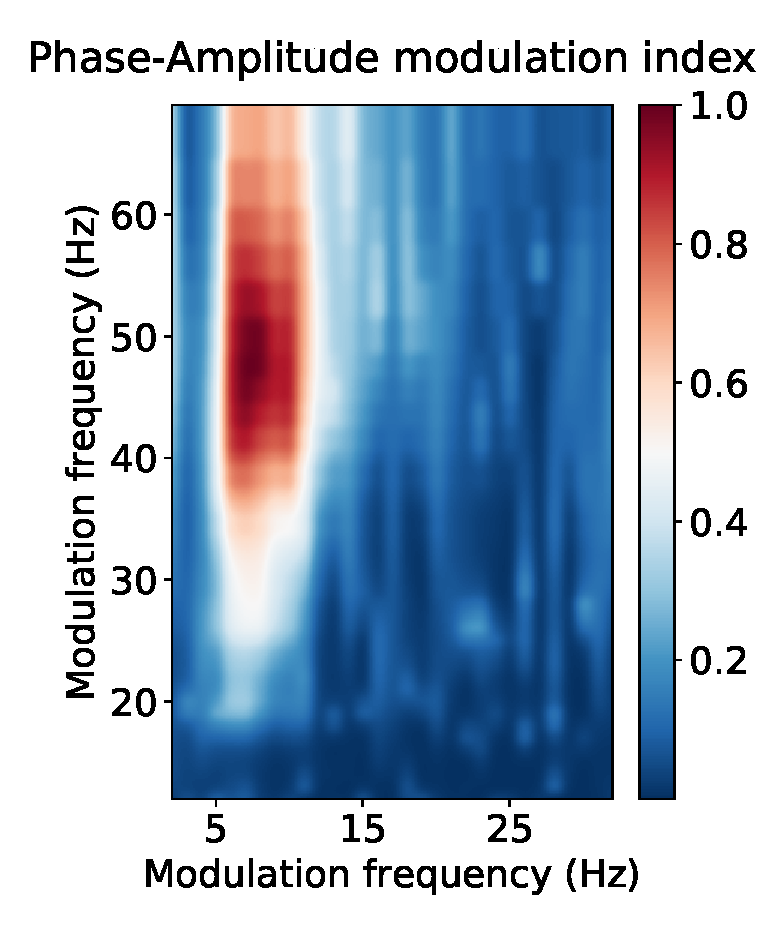
\includegraphics[width=\linewidth,keepaspectratio]{Modulation.eps}
% \endminipage
\begin{Figure}
\centering
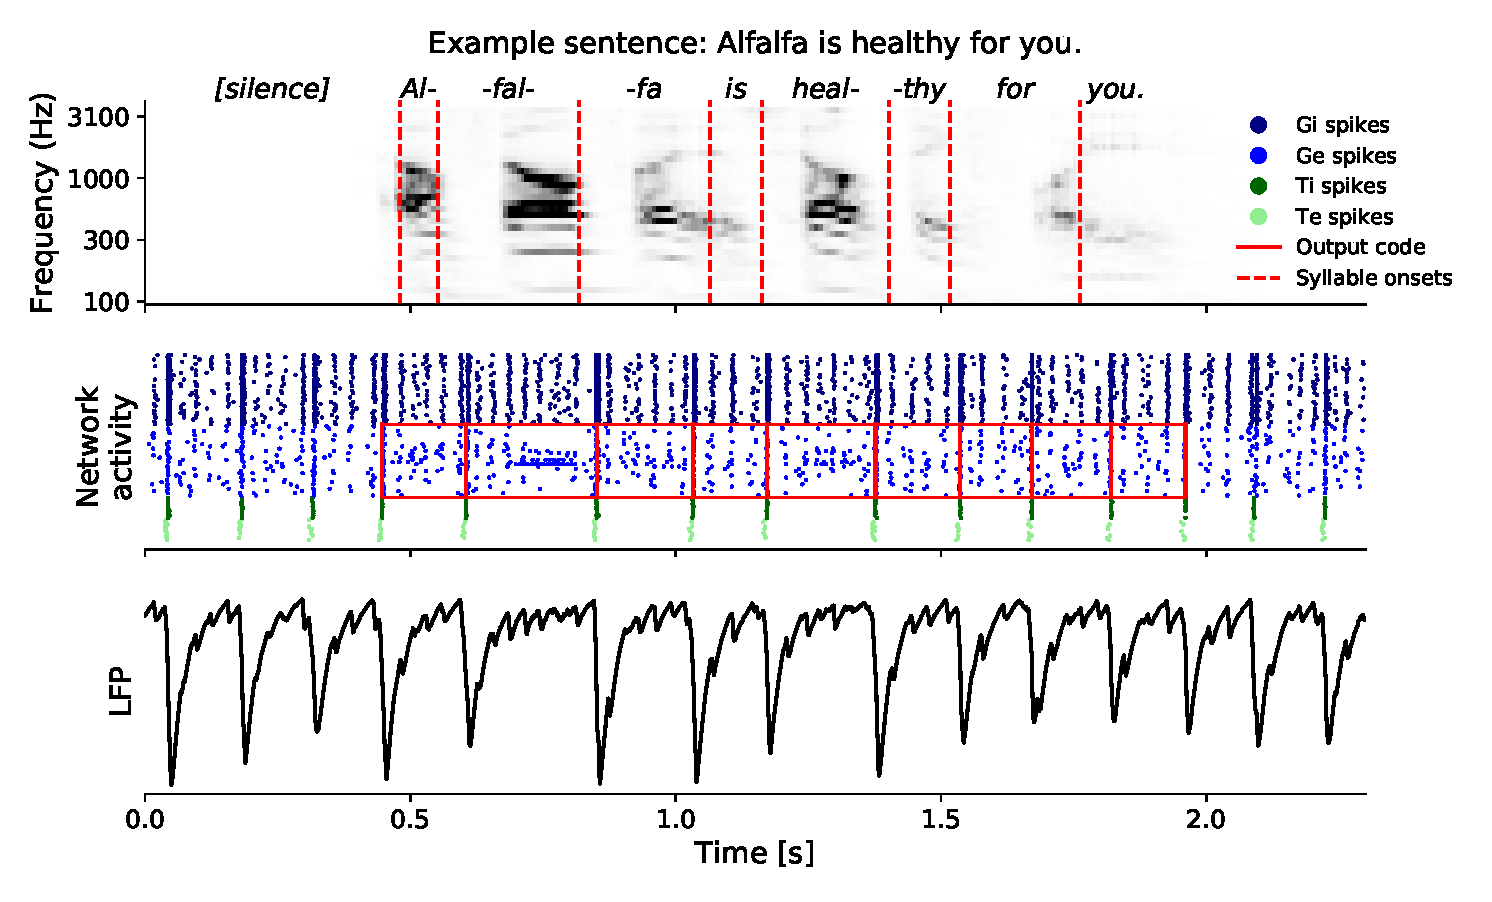
\includegraphics[width=\linewidth,keepaspectratio]{Behaviour_v2.eps}
\end{Figure}
\begin{flushleft}
\normalsize
The cross-frequency coupling provides strong modulation of the gamma activity by theta oscillations (middle and bottom panels). Spike bursts in PIN-TH network (green) are entrained to syllable onsets (red, dashed) and determine time-windows for the fast gamma activity (red, solid).
\end{flushleft}
% \minipage{0.7\linewidth}
% \endminipage\hfill
% \minipage{0.3\linewidth}
% \centering
% 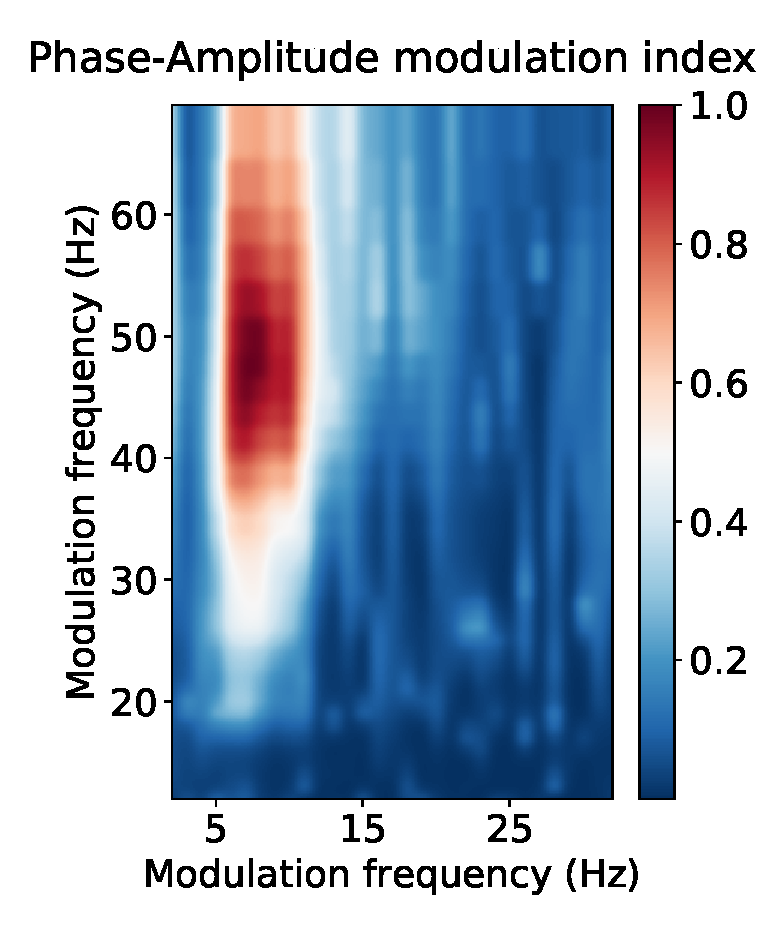
\includegraphics[width=\linewidth,keepaspectratio]{Modulation.eps}
% \endminipage
\subsection*{The effects of TES on LFP of the decoupled network at rest}
\begin{Figure}
\centering
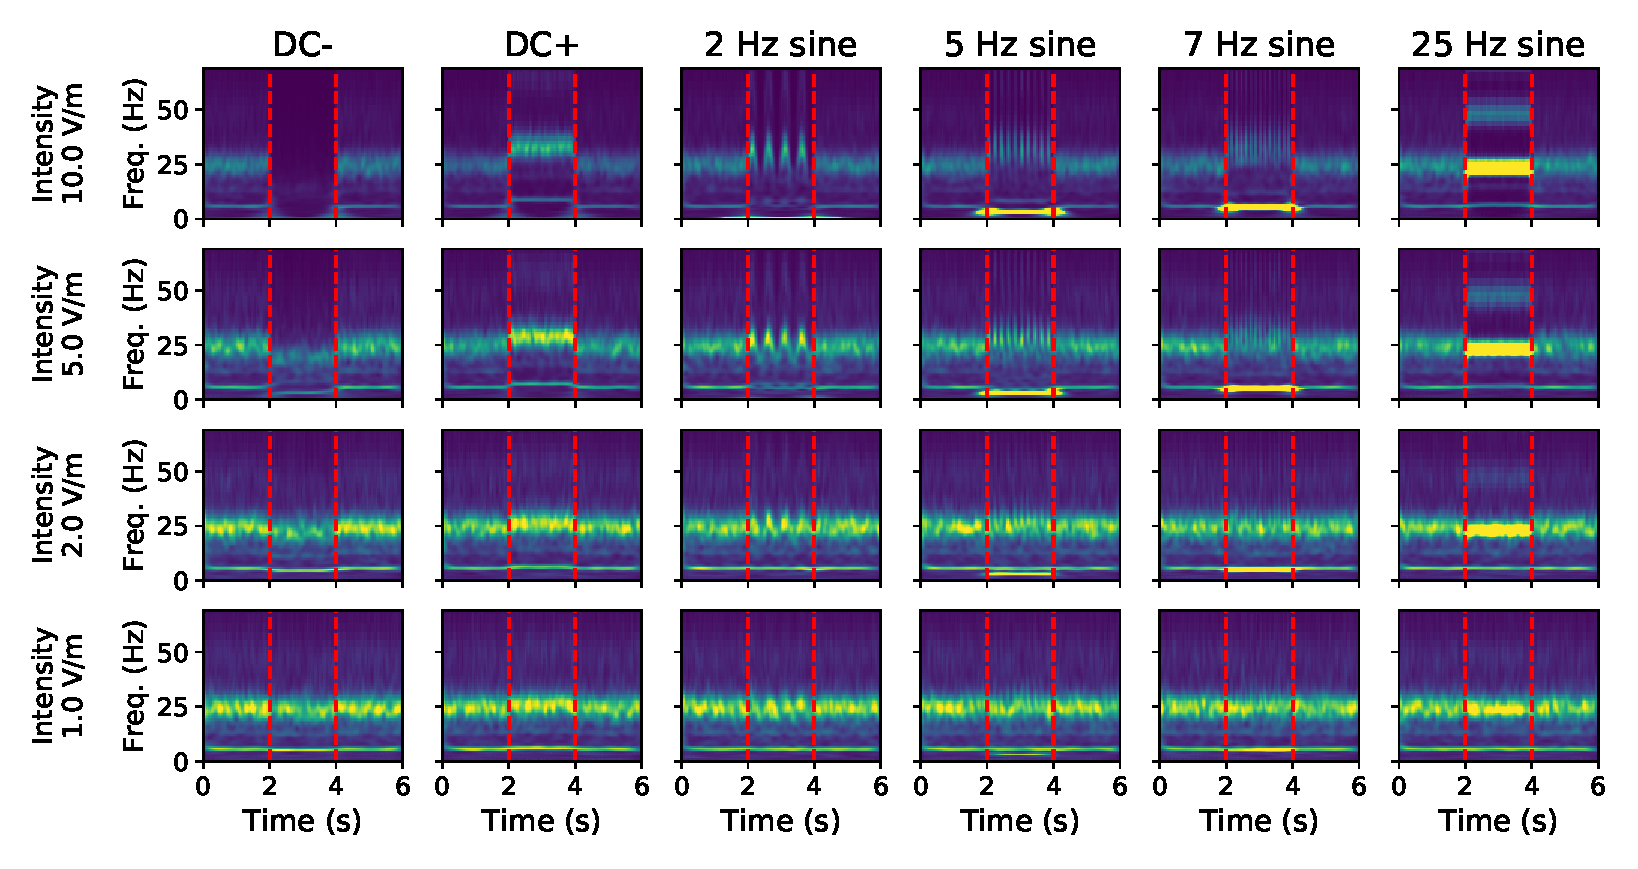
\includegraphics[width=\linewidth,keepaspectratio]{SimpleStim.eps}
\end{Figure}
\begin{flushleft}
\normalsize
%The cross-frequency coupling was removed to investigate the effects of TES on the LFP obtained from theta and gamma bands. 
The red dashed lines indicate the onsets and offsets of stimulation. For low-frequency TES (2-7 Hz), the gamma activity (20-40 Hz) was temporally modulated while the theta (6-9 Hz) was entrained to the stimulation frequency. The high-frequency TES almost exclusively affected the gamma activity.
\end{flushleft}
\subsection*{Speech-in-noise syllable decoding}
% \begin{Figure}
% \centering
% 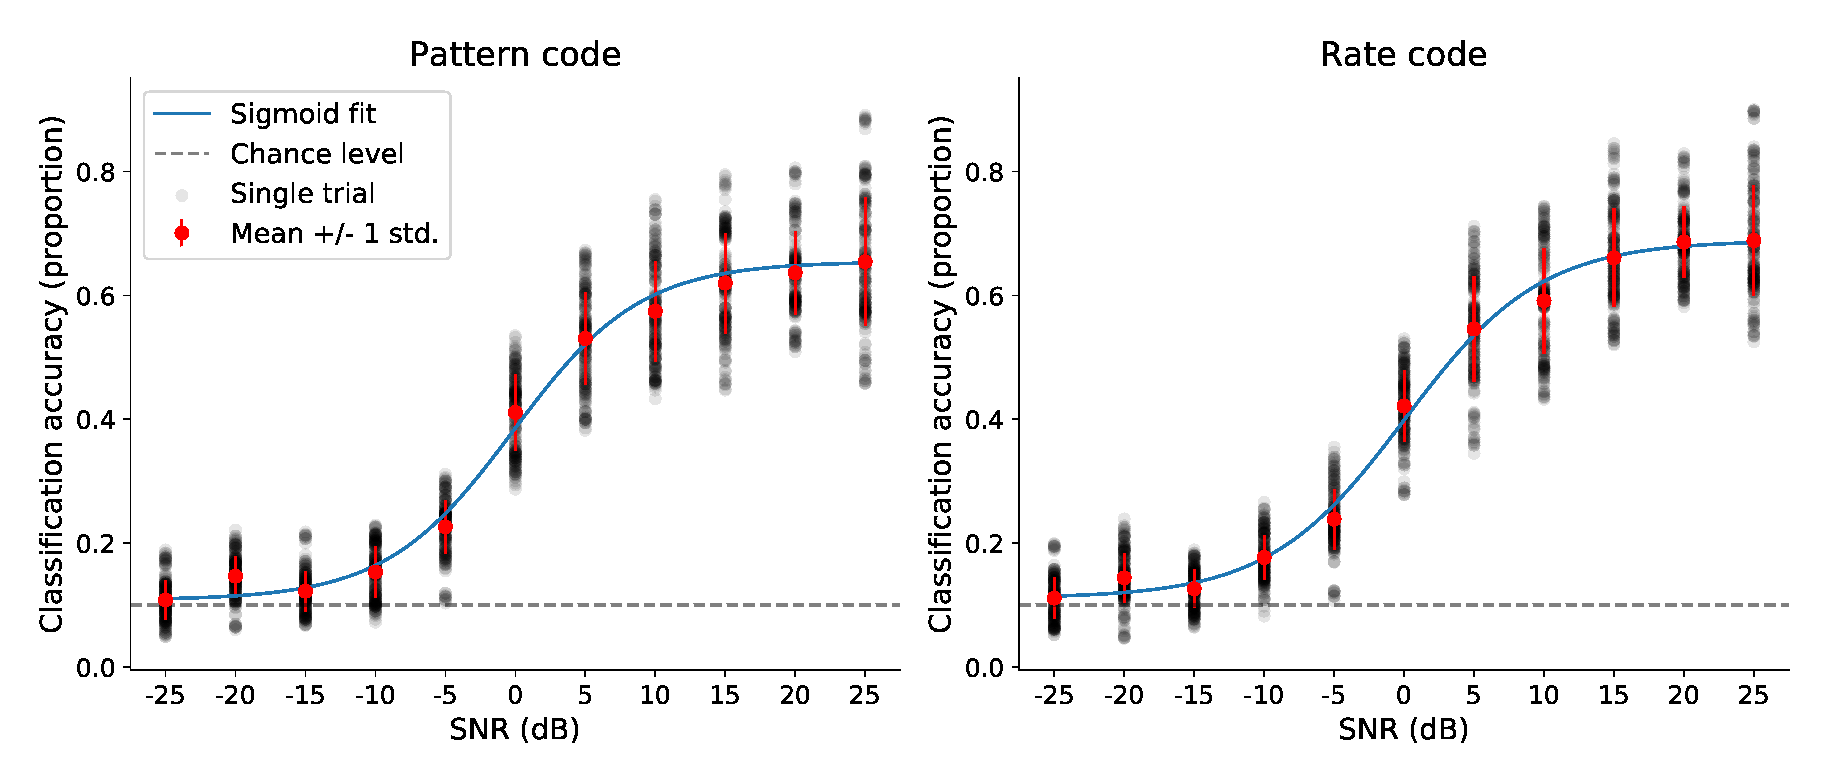
\includegraphics[width=\linewidth,keepaspectratio]{SNRdecoding.eps}
% \end{Figure}
\begin{Figure}
\centering
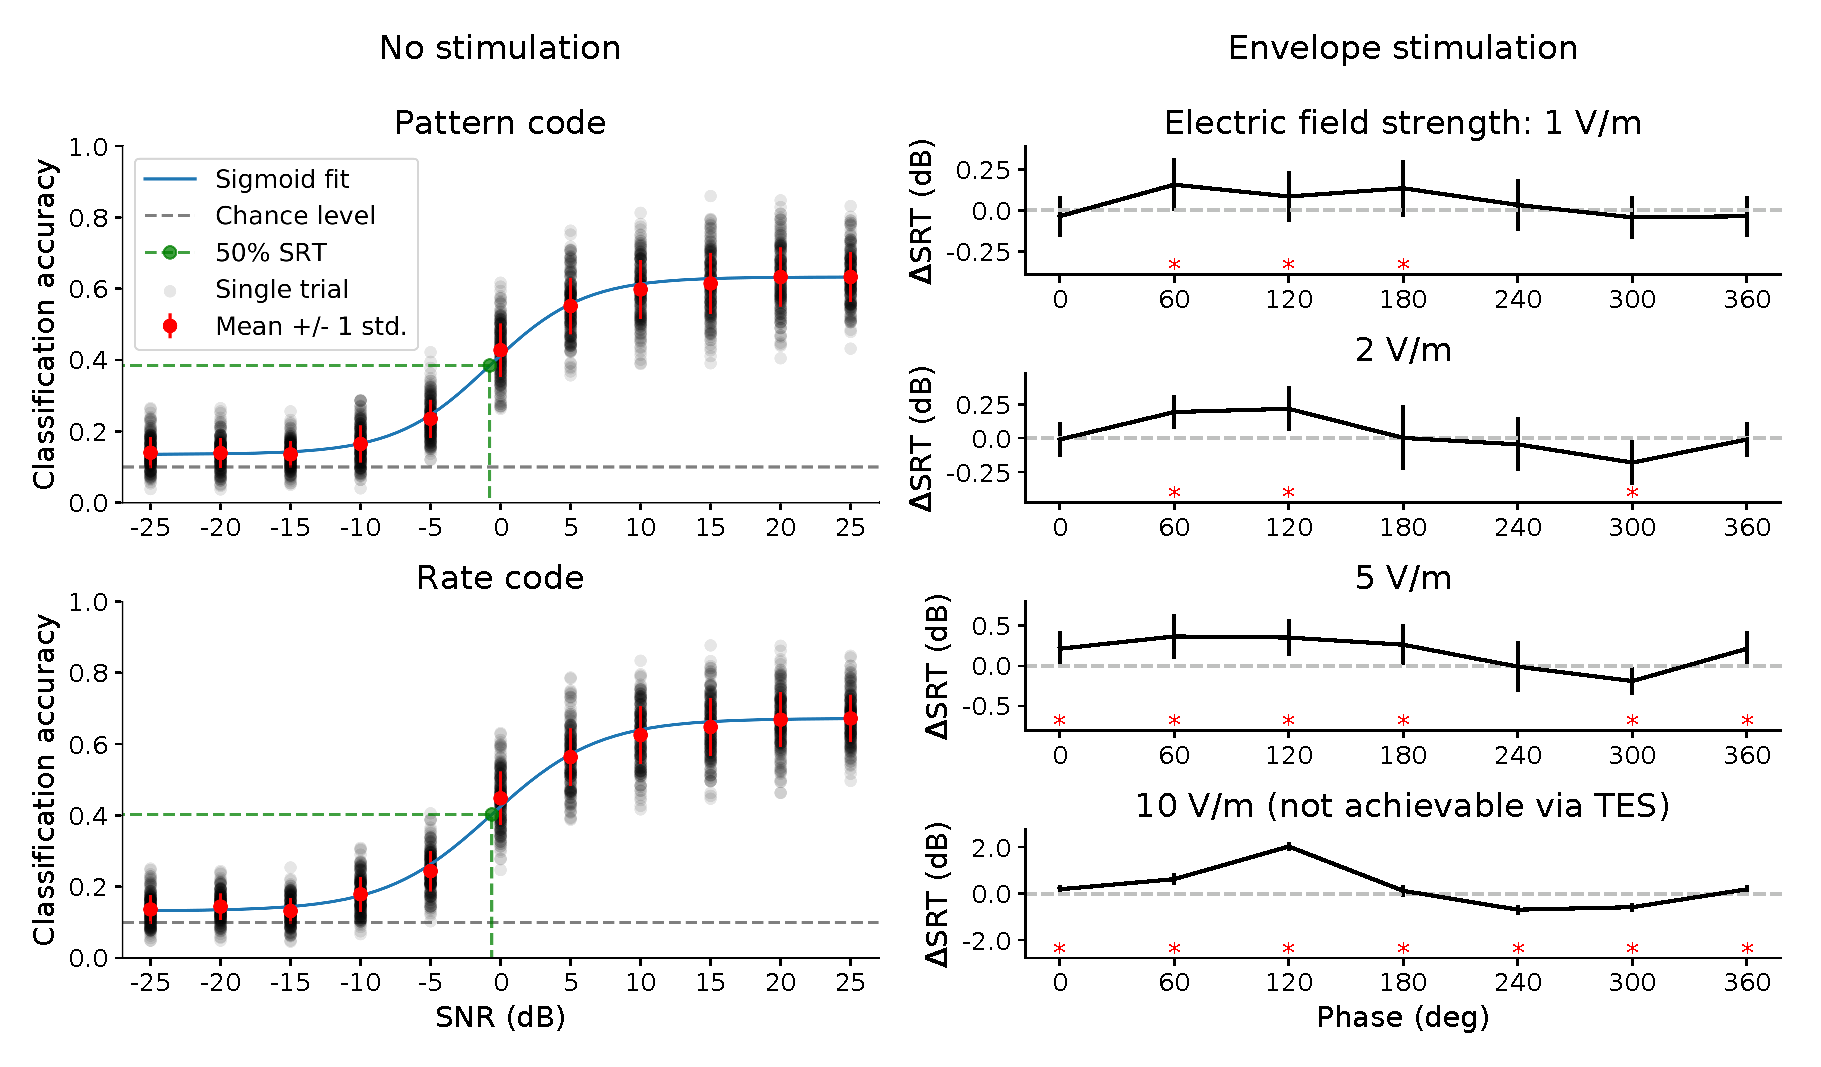
\includegraphics[width=\linewidth,keepaspectratio]{Stimulation.eps}
\end{Figure}
\begin{flushleft}
\normalsize
In agreement with the 50\% speech reception threshold (SRT) in normal hearing population, 50\% of the relative decoding accuracy, with no stimulation applied, was identified at -1 dB. The syllable decoding performance, measured as a shift of the 50\% SRT from the 'no stimulation' case (left), was significantly (p$<$0.05, red asterisk) modulated by certain phases of the envelope stimulation.
\end{flushleft}

% \subsection*{Modulation of speech-in-noise decoding via envelope TES}

% %\minipage{0.5\linewidth}

% %\endminipage\hfill
% %\minipage{0.5\linewidth}
% %\centering
% %\includegraphics[width=\linewidth,keepaspectratio]{EnvModulation_v2.eps}
% %\endminipage

% \begin{Figure}
% \centering
% \includegraphics[width=\linewidth,keepaspectratio]{EnvModulation_v3.eps}
% \end{Figure}
% \normalsize
% \begin{nitemize}
% \item The results obtained from stimulation conditions were compared to the case where no stimulation was applied (see above).
% \item The model speech-in-noise decoding performance was significantly (p $<$ 0.05, red asterisk) modulated by the certain phases of the applied envelope stimulation.
% \item The observed effects increased with the strength of the applied stimulation.
% \end{nitemize}

%----------------------------------------------------------------------------------------
%	CONCLUSIONS
%----------------------------------------------------------------------------------------
%\section*{\underline{Conclusion}}
%\begin{flushleft}
%\large
%The presented model can be used to classify syllables taken from spoken sentences with different levels of background noise. Model's relative decoding performance is comparable to normal human speech-in-noise perception with 50\% SRT at 0 dB.
%\end{flushleft}

%----------------------------------------------------------------------------------------
%	Next steps
%----------------------------------------------------------------------------------------

%\section*{\underline{Next steps}}
%\begin{flushleft}
%\large
%\begin{nitemize}
%\item Simulate the effect of different external currents on the network dynamics at rest and during speech encoding.
%\item Optimize the stimulation paradigm for enhancement of natural speech processing.
%\end{nitemize}
%\end{flushleft}

%----------------------------------------------------------------------------------------
%	ACKNOWLEDGEMENTS
%----------------------------------------------------------------------------------------

\small
\subsection*{Acknowledgements}
\begin{flushleft}
This study is supported by the EPSRC Centre for Doctoral Training in Neurotechnology for Life and Health. We thank Shabnam Kadir, Alexandre Hyafil and Milos Cernak for helpful comments and fruitful discussions. 
\end{flushleft}

%----------------------------------------------------------------------------------------
%	REFERENCES
%----------------------------------------------------------------------------------------
\subsection*{References}
\begingroup
\footnotesize
\renewcommand{\section}[2]{}%
\bibliographystyle{apalike}
\bibliography{Mendeley}
\endgroup
%----------------------------------------------------------------------------------------

\end{multicols*}
\end{document}